\documentclass{scrbook}

\usepackage{ngerman}
\usepackage{url}
\usepackage[pdfborder={0 0 0}]{hyperref}
\usepackage[utf8]{inputenc}
\usepackage{booktabs}
\usepackage{float}
\usepackage{listings}
\usepackage{xcolor}
\usepackage{graphicx}
\usepackage[nottoc,numbib]{tocbibind}
\usepackage[nonumberlist,acronym,section]{glossaries}

\definecolor{grau}{gray}{0.75}

\bibliographystyle{plain}

\title{Test Dokument}
\author{Dominik Meyer \url{dmeyer@hsu-hh.de}}
\makeglossary
\loadglsentries{acronyms}

\begin{document}

\maketitle
\newpage
\printglossary[type=\acronymtype,title=acronyms,style=long]
\listoffigures
\listoftables
\tableofcontents


\chapter{Kapitel}
\section{Kapitel}
\label{chap:kapitel:kapitel}

In Kapitel~\ref{chap:kapitel:kapitel} habe ich \ldots

Eine \gls{cpu} ist toll. Mit einer \gls{cpu} kann man viel machen.
\subsection{Unterkapitel}
\subsubsection{Hervorheben von Text}
\LARGE LARGE
\Large Large
\normalsize normal
\tiny tiny
\footnotesize footnote
\normalsize normal
\emph{Hallo} \textbf{Welt} ! \underline{Test}

Kühlschrank\footnote{was zum kühlen}.

\subsubsection{Itemize Umgebung}
\begin{itemize}
  \item item1
  \item item2
  \item item3
\end{itemize}

\subsubsection{enumerate Umgebung}

\begin{enumerate}
  \item item1
  \item item2
  \item item3
  \item \begin{enumerate}
    \item blah1
    \item blah2
    \item blah3
  \end{enumerate}
\end{enumerate}

\subsubsection{description Umgebung}

\begin{description}
\item[wort] erklärung
\item[2. wort] erklärung
\end{description}
\newpage
\subsection{Tabellen}

\begin{table}[htb]
\centering
\begin{tabular}{l|l|l}
\toprule
 \multicolumn{1}{c|}{\textbf{spalte1}} & \multicolumn{1}{c|}{\textbf{spalte2}} &
 \multicolumn{1}{c}{\textbf{spalte3}} \\ \midrule zeile1 spalte 1 & zeile1
 spalte 2 & zeile1 spalte 3 \\
zeile2 spalte 1 & zeile2 spalte 2 & zeile2 spalte 3 \\ 
\& & & \\
zeile3 spalte 1 & zeile3 spalte 2 & zeile3 spalte 3 \\
\bottomrule
\end{tabular}
\caption{Erste Tabelle}
\label{tab:erstetabelle}
\end{table}
In dfdsfdsfdsfdfsdfdsfds dsfsadfdsfds dsfsadfasdfsdfsdfsdfdsa adfdsf
adfadsfsafdsfs  Tabelle~\ref{tab:erstetabelle} wurde das und das beschrieben.

\subsection{Quellcode}
\lstset{language=C,commentstyle=\color{gray}\bfseries,keywordstyle=\color{blue},numbers=left,stepnumber=2,numberstyle=\tiny,frame=single,
captionpos=b}
\begin{lstlisting}[caption=mein erster Quellcode, label={lst:quellcode1}]
    int main() {
        int a=0; // variablen deklaration
    }
\end{lstlisting}

\subsubsection{include}
 \lstinputlisting[caption=mein zweiter Quellcode,
 label={lst:quellcode2}]{test.c}
 

In Listing~\ref{lst:quellcode1} oder \ref{lst:quellcode2} 

\subsection{Bilder}

\begin{figure}[htb]
\centering
%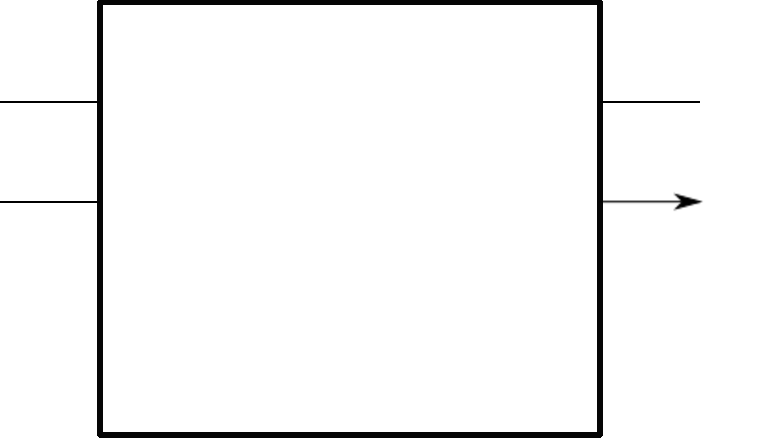
\includegraphics[height=0.5\textheight,angle=90]{test}
\caption{mein erstes Bild}
\label{fig:meinerstesBild}
\end{figure}

In Abbildung~\ref{fig:meinerstesBild}
\chapter{Kapitel}
\section{Kapitel}
\subsection{Unterkapitel}
\subsubsection{UnterUnterkapitel}
RS232 ist ein bekanntes Protokoll\cite{wiki:rs232}\ldots

\chapter{Kapitel}
\section{Kapitel}
\subsection{Unterkapitel}
\subsubsection{UnterUnterkapitel}

\bibliography{literatur}

\end{document}
